\chapter{SmartIO}\label{chapter:smartio}
SmartIO is a solution for allowing the local resources of a machine,~i.e., memory and devices, to be shared with and used by remote machines, over standard \gls{pcie}.
%
Our solution works for \emph{all} standard \gls{pcie} devices and their Linux device drivers, no special adaptation is needed in either hardware or software to make this sharing possible.
%
SmartIO is fully distributed and avoids dedicated servers.
%
All machines in the cluster~network may contribute their own local resources and access remote resources.
%
Furthermore, as remote devices and memory resources are accessed over native \gls{pcie}, they can be shared and used by remote machines with very low latency and extremely low computing overhead.
%
Whether devices are actually local or remote becomes irrelevant to the user, as SmartIO eliminates this distinction, with regard to both functionality and performance.
%
In other words, SmartIO is a flexible and efficient solution for scaling out and using more hardware resources than there are available in a single machine.


\section{Underlying idea}\label{sec:idea}
\begin{figure}
    \centering
    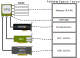
\includegraphics{bus-enumeration}
    \caption[Devices are mapped to the same address space as the \glsfmtshort{cpu} and system memory]
    {Device memory regions (\glsxtrshortpl{bar}) are mapped to the same address space as \glsxtrshort{cpu} and system memory, allowing
    the \gls{cpu} to read from and write to device memory the same way it would access \glsxtrshort{ram}. Devices can similarly use \gls{dma} to read from and write to \glsxtrshort{ram}.}
    \label{fig:bus-enumeration}
\end{figure}
The defining feature of \gls{pcie}~\cite{spec:PCIe} is that devices are mapped into the same address space as the \gls{cpu} and \gls{ram}, as seen in \cref{fig:bus-enumeration}.
%
This allows a \gls{cpu} to read from and write to device memory in the same manner it would access \gls{ram}, also known as \gls{mmio}.
%
Likewise, devices capable of \gls{dma} may read from and write to \gls{ram} directly.
%
\Gls{pcie} also uses \gls{msi}, allowing devices to raise interrupts by writing to an address reserved by the \gls{cpu} instead of requiring dedicated interrupt lines.



This address space mapping occurs when a system enumerates the \gls{pcie} bus and accesses the \gls{cfgspace} of each device.
%
A \gls{cfgspace} contains a description of the capabilities of a device, such as its memory regions.
%
The system will reserve a memory address range for each of these device memory regions, and by writing the start address of these regions to the device's \glspl{bar}, a device is made aware of the address space mapping.
%
Therefore, the term ``\gls{bar}'' is used interchangeably for a region of device memory.
%
Addresses reserved by the system for interrupts are also written to the device's \gls{cfgspace}.
%
For more details on \gls{pcie}, particularly how memory transactions are routed, please refer to \paperref{tocs:pcie,cc:pcie}.



\begin{figure}
    \centering
    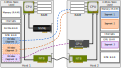
\includegraphics[width=.99\textwidth]{ntb-example}
    \caption[Two computer systems connected using \glsfmtshortpl{ntb}, and the \glsfmtshortpl{ntb} translate between the two different address domains]
    {Two computer systems connected together using \glspl{ntb} and external cables. Host~1 has mapped \glspl{segment} of Host~2's memory through its local \gls{ntb}, providing Host~1 with ``windows'' into the remote system's address space. The \glspl{ntb} translate addresses between the two independent address spaces.}
    \label{fig:ntb-example}
\end{figure}



As depicted in \cref{fig:ntb-example}, it is possible to connect computer systems with different address spaces together over \gls{pcie} by using \glspl{ntb}.
%
\Glspl{ntb} can be embedded as a \gls{cpu} feature~\cite{whitepaper:Sullivan2010,url:LinuxNTB-AMD}, but are more commonly implemented in \gls{pcie} switch chips~\cite{whitepaper:PLX,pex8733}.
%
By using such \gls{ntb}-capable switch chips to implement peripheral devices, independent computer systems can connect with plug-in host adapter cards and external cables.
%
To the system, the \gls{ntb} appears as a normal \gls{pcie} device\footnote{The \gls{pcie} terminology for individual \glspl{devicefunction} is ``\glspl{ep}''. We use the terms ``device'' and ``\gls{function}'' as synonyms for a \gls{pcie} \gls{ep} throughout this dissertation.} with one or more \glspl{bar} that are reserved and mapped during the enumeration process.
%
However, rather than being backed by device registers or device memory, the \gls{ntb} instead forwards reads and writes to its \glspl{bar} from one side of the \gls{ntb} to the other, translating memory addresses in the process.
%
The \gls{ntb} uses a \gls{lut} for address translation, which can be configured dynamically during run-time.
%
By using different base offsets in this \gls{lut}, it is possible to configure several memory-mappings (or ``windows'') into the address space of a remote system.
%
\Cref{fig:ntb-example} illustrates how arbitrary memory addresses on the remote system can be mapped, allowing the local \gls{cpu} to access remote memory as if it was local device memory.
%
Although address translation between the different address spaces is very fast since the \gls{lut} is implemented in \gls{ntb} hardware, the number of \gls{ntb} windows is limited by the maximum number of table entries.
%
More details on how \glspl{ntb} work can be found in \paperref{tocs:pcie-ntb}.



Since device memory on a remote system is part of the same address space as system memory, we can use an \gls{ntb} to map memory of a remote device.
%
We show this in \cref{fig:ntb-example}, where Segment~3 is allocated in \gls{gpu} memory rather than system~\gls{ram}, but still mapped for the \gls{cpu} of Host~1's similarly to the other \glspl{segment}.
%
By mapping all \glspl{bar} of a remote device for a local \gls{cpu}, it would be possible to perform memory operations on the remote device, such as reading from or writing to device registers.
%
Moreover, device~\gls{dma} is not limited to reading and writing to system \gls{ram}, but can also be used to access memory on other devices in the same address space.
%
This is known as ``\gls{p2p}'' in \gls{pcie}, and provides us with an opportunity as it becomes possible for a device to read and write directly across an \gls{ntb}.
%
We can use this to map memory resources for a device, be it \gls{ram} or memory of other devices. 
%
Furthermore, because \gls{pcie} uses \gls{msi}, it is even possible to map interrupt addresses through an \gls{ntb}, as they too are mappable.




\section{Main challenges}\label{sec:challenges}
Although \glspl{ntb} provide the fundamental memory mapping capabilities that can facilitate the use of remote devices, the challenge is to avoid requiring device drivers to be aware of remote-side address spaces.
%
As touched upon in \cref{sec:motivation}, this is desirable in order to use existing device driver implementations.
%
In order for a device driver running on a local~machine to use a remote~device, we must make sure that the driver uses addresses that is mapped through both the local and remote \glspl{ntb}.
%
For instance, when the device driver attempts to access \glspl{devicebar}, we must make sure that the driver uses memory addresses that are mapped through the \gls{cpu}-side \gls{ntb} without the driver or device being aware of this.
%
Conversely, when the device driver attempts to initiate \gls{dma} transfers or configures an interrupt vector address, we must find a way to transparently inject memory addresses that are mapped through the remote, or device-side, \gls{ntb}.



One possibility is to use virtualization to mitigate the complexity of managing different address spaces.
%
The fact that devices are on the other side of an \gls{ntb} could be hidden for device drivers by distributing devices to \gls{vm} \glspl{guest} instead of physical \lgls{host}{host~machines}, for example with \gls{passthrough}.
%
However, while \gls{passthrough} allows devices to be used by \glspl{vmguest} directly, requiring that compute tasks run in \glspl{vm} limits the generality of a solution.
%
Virtualization is not necessarily appropriate in all circumstances, as it may add additional system load because \gls{cpu} cycles are spent on \lgls{host}{hosting} the virtualized environment.
%
A more general mechanism is needed for abstracting away the complexity of dealing with a remote-side address space, in order to support sharing to bare-metal machines in addition to \glspl{vm}.



\Gls{dma} is particularly challenging in this context.
%
A device driver running on the \gls{hostmachine} may assume that any local memory address can be reached by the device, but as explained in \cref{sec:idea}, the \gls{ntb} only provide \emph{windows} into a remote address space.
%
It is generally not possible to predict in advance which memory addresses a device driver may use, yet memory must be mapped through the \gls{ntb} before the driver, unaware that the device is remote, initiates \gls{dma} transfers.
%
Deferring the action of mapping memory through the \gls{ntb} until a device driver initiates \gls{dma}, or some other time when the specific addresses of \gls{dma} buffers and \gls{vm} memory can be known, is not viable;
%
synchronizing with the remote system at this time will introduce communication overhead in the performance-critical path.
%
The naive solution is to map the entire system memory for the device, but this workaround requires the \gls{ntb}~\glspl{bar} to be at least \emph{as large} as the size of \gls{ram}.
%
This does not scale very well, as it would effectively limit the number of machines the cluster can support;
%
each machine added would increase the \gls{ntb} memory requirements by its entire \gls{ram} size.
%
Moreover, the number of maps supported by an \gls{ntb} is also limited (by the size of its \gls{lut}).
%
We must find a way to prepare memory-maps through the \gls{ntb} in advance of use, in order to avoid adding communication latency in the critical path, and without requiring that the entire memory is mapped for the device.



The challenge of \gls{dma} transfers is compounded for \gls{vmpassthrough}.
%
\Gls{passthrough} is possible by using the \gls{iommu} to create a virtual \gls{io} address space for a device that corresponds to the virtual address space of the \gls{vm}~\cite{url:LinuxVFIO,url:LinuxIOMMU,Muli2006}, also known as the ``\gls{guestphys} address space''.
%
However, in order for a remote device to reach local \gls{hostphys} memory, it must use addresses that are mapped through the \gls{ntb}.
%
A device driver running in the \gls{vmguest} on the local \gls{host} may try to use any (virtualized) memory address when initiating \gls{dma} transfers.
%
Consequently, supporting \gls{passthrough} requires devising a method for mapping the physical memory backing the \gls{vmemulator} through the \gls{ntb}, using device-side \gls{io} addresses that mirrors the \gls{guestphys} address space.



The published papers provide further details on the challenges facing our solution as part of the description of the implementation of the different components of SmartIO.
%
Particularly \paperref{tocs:lending,tocs:mdev,tocs:nvme} provide a more in-depth explanation of what the main challenges are, and they also explain how SmartIO tackle them.
%
A discussion of additional considerations is given in \paperref{tocs:disc}.



\section{Implementation}\label{sec:implementation}
In our framework, computer systems act as \emph{``\glspl{borrower}''} and \emph{``\glspl{lender}''}.
%
A \gls{lender} is a computer system that registers one or more of its internal \gls{pcie} devices with SmartIO, allowing these devices to be distributed to and used by remote machines.
%
A \gls{borrower} is a system that is currently using such a device. 
%
While a device only has one \gls{lender}, namely the computer system where it is physically installed, there can be several \glspl{borrower} using it simultaneously.
%
SmartIO also makes it possible for a system to act as both \gls{lender} and \gls{borrower} at the same time, lending out its own local devices and simultaneously borrowing remote devices from other machines.



Basing our framework on standard \gls{pcie} is a a crucial part of the design.
%
Not only does this allow commodity devices to be operated remotely by standard device drivers over native \gls{pcie}, but this design also means that the implementation complexity of SmartIO lies entirely in software.
%
In fact, SmartIO can be implemented for existing computer systems that are connected using \glspl{ntb} in any network topology, regardless of whether the \glspl{ntb} are switch chips soldered onto a motherboard or implemented as plug-in adapter cards.



Unlike other solutions for distributed \gls{io}, SmartIO combines traditional \gls{io} with distributed shared-memory functionality in a seamless manner.
%
Sharing is supported at multiple abstraction levels:
%
devices may be distributed to physical \glspl{hostmachine} and to \glspl{vm} alike.
%
Individual \lgls{function}{device functions} of \lgls{function}{multi-function} devices may be distributed to different machines in the network, or to the same machine should it require multiple resources.
%
SmartIO also provides software facilities for \gls{disaggregating} devices and memory resources, allowing device drivers to be implemented as part of distributed cluster applications or other \gls{userspace} applications. 
%
This makes it possible for several machines to simultaneously share a single \lgls{function}{device~(function)}.
%
It is even possible to \emph{combine} the sharing methods of SmartIO. 
%
For example, we can \gls{disaggregate} the device memory of a remote \gls{gpu} using the \gls{apiext} while it is being borrowed through \gls{dl}, or we can share \glspl{vf} of an \gls{sriov} \gls{nic} with both physical \glspl{hostmachine} and \glspl{vm}.


\begin{figure}
    \centering
    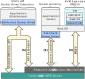
\includegraphics{software-architecture}
    \caption[Three different sharing methods are made possible by our framework. The SmartIO driver abstracts away the physical location of a remote resource]
    {The software architecture of SmartIO. Three different sharing methods are made possible by our framework: \textbf{(1)}~\gls{dl}, \textbf{(2)}~\gls{mdev}, and \textbf{(3)}~using the \gls{sisciapiext}. The SmartIO driver, shown as layer \textbf{(B)}, abstracts away the physical location of remote resources, for both the shared device and software using the device.}
    \label{fig:architecture}
\end{figure}


In this section we address the challenges of \cref{sec:challenges}, and give a bottom-up summary of the implementation of SmartIO.
%
\cref{fig:architecture} illustrates the different components of our framework, and how they fit together.
%
The full implementation details can be found in the published papers, with \cref{paper:tocs} providing a detailed description of the entire solution as a whole.



\subsection{Low-level NTB driver}\label{sec:ntb-driver}
SmartIO is implemented on top of the \gls{ntb} interconnection solution from Dolphin.
%
The low-level \gls{ntb} driver, illustrated as layer \textbf{(A)} in \cref{fig:architecture}, provides the fundamental \gls{pcie} networking infrastructure and memory mapping functionality which SmartIO builds on.
%
Individual systems may contribute parts, or \emph{\glspl{segment}}, of their local memory to a distributed, shared memory space. 
%
\Glspl{memorysegment} in remote machines may be mapped into the local address space of a system by using the \gls{ntb}, as explained in \cref{sec:idea}.
%
Moreover, \gls{userspace} applications may use the \gls{sisciapi} to interact with the \gls{ntb} driver to manage \glspl{memorysegment} and implement shared-memory communication.



\subsection{SmartIO driver}\label{sec:smartio-driver}
The SmartIO driver, shown as layer \textbf{(B)} in \cref{fig:architecture}, runs on all machines in the cluster.
%
It acts as an abstraction layer, providing a logical decoupling of devices and which physical machines they are installed in (\glspl{lender}).
%
Neither devices nor software need to consider where resources physically reside, since SmartIO resolves this on behalf of both devices and a machines using them (\glspl{borrower}).
%
By providing this abstraction, the SmartIO driver is the first step towards \gls{dl}, \gls{mdev}, and the \gls{sisciapiext}, presented in \cref{sec:lending,sec:mdev,sec:api} respectively.


Devices registered with SmartIO are assigned a unique identifier which allows machines to refer to a device without needing to specify the \gls{lendermachine}.
%
Internally, the SmartIO driver keeps track of devices and \glspl{lender}, and uses this device identifier to look up machines, devices, and which \gls{ntb} to use.
%
The SmartIO driver is also responsible for making \glspl{devicebar} available as \glspl{sharedsegment}, making it possible for \glspl{borrowermachine} to memory map remote device memory into their local address space (\gls{mmio}).



Most important is the SmartIO driver's responsibility of mapping \glspl{memorysegment} \textbf{on behalf of a device} and returning the \gls{io} addresses to these maps, \textbf{as seen by the device}.
%
The SmartIO driver works out the physical locations of devices and \glspl{memorysegment},~i.e., which machines they reside in and which \glspl{ntb} a device must use in order to reach a \gls{segment}.
%
Note that a \gls{segment} can reside in memory of the machine using the device~(the \gls{borrower}), in memory of the machine where the device is installed~(the \gls{lender}), or a different cluster machine altogether.
%
A segment can even be allocated in device memory of another device, as the SmartIO driver can assist in mapping device \glspl{bar} and enabling \gls{p2p} between devices.
%
\Glspl{borrower} are not required to know anything about the \emph{device-side} \gls{io} addresses returned by our SmartIO driver, other than the fact that they resolve to the same address space as the device.
%
This allows both a \gls{borrower} and the device to remain agnostic about the underlying, physical \gls{pcie} topology, as they can rely on the SmartIO driver to resolve paths in the cluster network and map resources through the appropriate \glspl{ntb}.



The SmartIO driver solves the challenge of managing multiple address spaces, as described in \cref{sec:challenges}.
%
For example, a \gls{borrower} can request a \gls{memorysegment} in a different machine is mapped so that the device may use \gls{dma} to it.
%
Our SmartIO driver will look up which machine the \gls{memorysegment} is in, look up the \gls{lendermachine} and which (device-side) \gls{ntb} it must use, configure the \gls{ntb}, map the \gls{memorysegment} for the device, and return the device-side \gls{io} address of this map back to the \gls{borrower}.
%
The \gls{borrower} can then use this \gls{io} address when interacting with the device in order to initiate the \gls{dma} transfer, and the device is able to reach the \gls{memorysegment} through the lender's \gls{ntb}.
%
\Glspl{borrower} do not need to be aware of the internal \gls{io} address space layout of a \gls{lender}.
%
As it happens, \glspl{borrower} do not even need to know which physical machine the \gls{lender} is.



With the abstraction the SmartIO driver provides, our framework is able to facilitate the sharing and use of remote resources (both memory and devices) as described in \cref{sec:lending,sec:mdev,sec:api}.
%
More details on how SmartIO resolves the paths between devices and other memory resources that must be mapped (for devices) are given in the papers, particularly in \paperref{tocs}.
%
However, please note that the SmartIO driver is not mentioned explicitly by name in the papers, as it is the unifying base for the sharing methods.
%
Instead, the description of its functionality is interleaved with the implementation details of these methods.



\subsection{Device Lending}\label{sec:lending}
\Gls{dl}, illustrated as arrow \textbf{(1)} in \cref{fig:architecture}, makes it possible to share and distribute devices to remote \glspl{hostmachine}.
%
The devices become part of the system they are shared with, allowing application software, device drivers, and even the \gls{os} to use them as if they were locally installed.
%
While \gls{dl} only allows individual \glspl{devicefunction} to be distributed to a single machine at the time, it is nevertheless highly suitable in the case where a device has a complex or proprietary device driver as no modifications to existing software is required.


As mentioned in \cref{sec:idea}, it is possible to map the device memory regions, or \glspl{bar}, of a remote device through an \gls{ntb}.
%
Using the \gls{ntb}, a local \gls{cpu} can perform memory operations on a remote device, such as reading from and writing to device registers.
%
Conversely, local resources, such as \gls{ram} and interrupt addresses, can in turn be mapped for the remote device itself. 
%
This allows the remote device to use \gls{dma} through the \gls{ntb} and trigger interrupt routines on the local \gls{cpu}.
%
The SmartIO driver, as explained in \cref{sec:smartio-driver}, eliminates the complexity of managing multiple address spaces: a user may rely on the SmartIO driver to map resources through the appropriate \glspl{ntb} and provide \gls{io} addresses corresponding to a device's address space.
%
However, as pointed out in \cref{sec:challenges}, we still need to make sure that device drivers use this functionality without requiring that they be re-written. 
%
More precisely, we need a mechanism for \emph{transparently} injecting resolved \gls{io} addresses, without the devices or their drivers being aware of this.



\begin{figure}
    \centering
    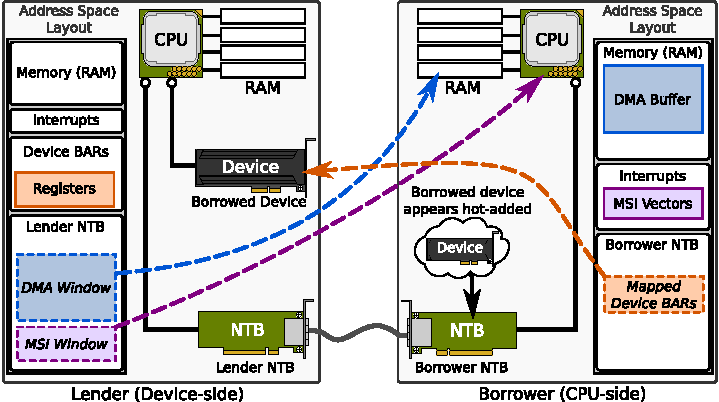
\includegraphics[width=.99\textwidth]{device-lending}
    \caption
    [The memory regions of a remote device is mapped for the \glsfmtshort{cpu} on the borrower, so that it can read and write to device registers. Local resources are mapped for the device, so that it may use \glsfmtshort{dma} and trigger interrupts. \Glsentrytext{dl} inserts a \glsentrytext{shadowdev} into the local device tree using these mappings, making remote device access transparent to both \glsfmtshort{cpu} and device.]
    {The memory regions of a remote device is mapped for the \gls{cpu} on the borrower, so that it can read and write to device registers. Local resources are mapped for the device, so that it may use \gls{dma} and trigger interrupts. \Gls{dl} inserts a \gls{shadowdev} into the local device tree using these mappings, making remote device access transparent to both \gls{cpu} and device.}
    \label{fig:device-lending}
\end{figure}


\Gls{dl} solves this by inserting a ``\gls{shadowdev}'' into the local \gls{pcie} device tree on the \gls{borrower}, as depicted in \cref{fig:device-lending}. 
%
The \gls{shadowdev} makes it appear as if the remote device has been \gls{hotadded} to the local system, and provides us with a mechanism for intercepting interactions with the device by the \gls{os} and any device drivers. 
%
We make sure that a device driver attempting to memory map the device's \glspl{bar} use addresses that map through the \gls{ntb}, without the driver being aware that the device is actually remote.
%
Similarly, when the device driver configures interrupts, we are able to intercept this and inject an address that map through the \gls{lender}'s \gls{ntb}, again without the driver being aware.



\begin{figure}
    \centering
    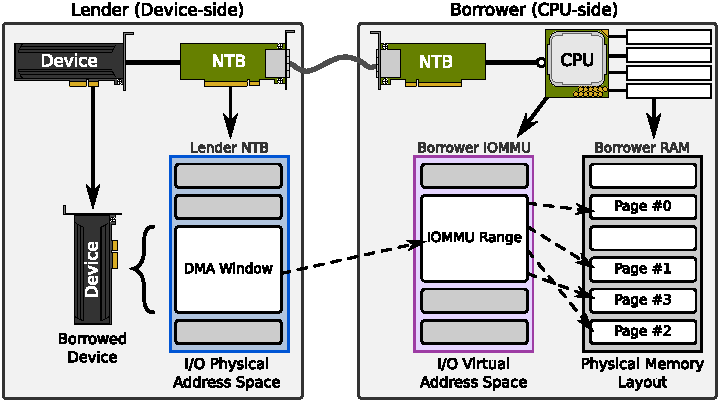
\includegraphics[width=.99\textwidth]{dma-window}
    \caption[The borrower's \glsfmtshort{iommu} is used to create a single continuous memory range that may be mapped through the lender's \glsfmtshort{ntb} in advance. Adding and removing memory pages from the local \glsfmtshort{iommu} domain is inexpensive compared to actively communicating with the remote lender~machine]
    {The \gls{borrower}'s \gls{iommu} is used to create a single continuous memory range that may be mapped through the \gls{lender}'s \gls{ntb} in advance. Adding and removing memory pages from the local \gls{iommu} domain is inexpensive compared to actively communicating with the remote \gls{lendermachine}.}
    \label{fig:dma-window}
\end{figure}


The \gls{shadowdev} also provides us with the means to detect when a device driver is allocating \gls{dma} buffers and making memory available for \gls{dma} transfers.
%
Unlike \glspl{devicebar} and \gls{msi} addresses, memory addresses for \gls{dma} buffers are not known in advance, as mentioned in \cref{sec:challenges}.
%
Mapping \glspl{bar} and interrupts is a one-time operation.
%
The pages used for \gls{dma} memory buffers, however, may be scattered in physical memory.
%
A driver may even initiate several transfers to different parts of memory altogether.
%
Mapping individual memory pages through the \gls{lender}'s \gls{ntb} would not only exhaust the number of available entries in its \gls{lut}, but communicating with the \gls{lendermachine} in order to map these pages dynamically would introduce communication latency in the critical performance path.



To solve this, \gls{dl} relies on the \gls{iommu} on the \gls{borrower}, as depicted in \cref{fig:dma-window}.
%
We can prepare a continuous memory address range \emph{in advance} using the \gls{borrower}'s \gls{iommu}.
%
This range can be mapped through the \gls{lender}'s \gls{ntb} with a single map, or ``\gls{dmawindow}'', even before any device drivers are using the device.
%
When a device driver, at a later point, allocates \gls{dma} buffers, we can simply add these addresses to the \gls{iommu} range.
%
This way, we can avoid making any assumptions about the memory used by a device driver.
%
Additionally, since this is an entirely local operation (on the \gls{borrower}), communication with the remote \gls{lendermachine} is avoided.
%
All address translations between the different address domains are done in \gls{ntb} and \gls{iommu} hardware, ensuring that this solution is able to achieve native \gls{pcie} performance in the data path.



A more technical description of the implementation of \gls{dl} can be found in \paperref{tocs:lending}, including details about the \gls{shadowdev} and \glspl{cfgcycle}.
%
\paperref{tocs:lending-p2p,cc:p2p} explain how \gls{dl} is able to support \gls{p2p} \gls{dma} between multiple borrowed devices, even when they reside in different \glspl{lendermachine}.
%
In addition, \paperref{tocs:lending-dma,tocs:disc-devs} explain how we can use the \emph{\gls{lender}'s} \gls{iommu} to remap \glspl{dmawindow} from high to low memory addresses for devices with addressing limitations.



\subsection{MDEV}\label{sec:mdev}
Our \gls{mdev} implementation, shown as arrow \textbf{(2)} in \cref{fig:architecture}, enables the Linux~\gls{kvm} to \emph{\lgls{passthrough}{pass through}} borrowed devices to \glspl{vm}.
%
This \gls{passthrough} makes it possible for software running in a \gls{vmguest} to use the physical device directly, without compromising the memory isolation provided by the virtualization.
%
As devices are no longer tightly coupled with the \glspl{hostmachine} they are installed in, \gls{mdev} makes it possible to distribute \glspl{vm} across different \glspl{host} in the cluster while benefiting from the bare-metal performance of direct access to physical hardware.

\begin{figure}
    \centering
    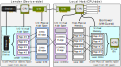
\includegraphics[width=.99\textwidth]{mdev-dma}
    \caption
    [The \glsfmtshortpl{iommu} on both sides of the \glsfmtshort{ntb} must be used in order to pass through a remote device to a local \glsfmtshort{vm}. The borrower's \glsfmtshort{iommu} is used to provide continuous memory ranges for scattered \glsfmtshort{vm} memory, while the lenders's \glsfmtshort{iommu} is used to mirror the guest-physical layout for the device]
    {The \glspl{iommu} on both sides of the \gls{ntb} must be used in order to \lgls{passthrough}{pass through} a remote device to a local \gls{vm}. The \gls{borrower}'s \gls{iommu} is used to provide continuous memory ranges for scattered \gls{vm} memory, while the \gls{lender}'s \gls{iommu} is used to mirror the \gls{guestphys} layout for the device.}
    \label{fig:mdev-dma}
\end{figure}


Our \gls{mdev} sharing method is implemented using the mediated device driver \gls{paravirtualization} interface~\cite{url:LinuxMDEV}.
%
Comparable to the \gls{shadowdev} used by \gls{dl}~(\cref{sec:lending}), this interface makes it possible to \gls{trap}~(handle) certain operations, such as \glspl{cfgcycle} and device resets, and to set the memory addresses of the device's \glspl{bar}.
%
However, unlike \gls{dl}, we do not have any means of controlling which \gls{io} addresses a device driver should use when initiating \gls{dma} transfers.
%
In \gls{dl}, we create a single, continuous \gls{iommu} range ahead of time, and map it through the \gls{lender}'s \gls{ntb}. 
%
We are able to detect when a device driver is preparing \gls{dma} buffers through the \gls{shadowdev}, and can inject the prepared device-side \gls{io} address of our \gls{dmawindow}.
%
In contrast, a device driver running in the \gls{vmguest} is completely isolated, leaving us without any equivalent mechanism to inject \gls{io} addresses we can control.
%
The only possible option is to make sure that the device is mapped to the same virtual address space as the \gls{vm}, as pointed out in \cref{sec:challenges}.



In order for a device to \gls{dma} to \gls{vm} memory, the \gls{hostphys} memory pages backing the emulated memory needs to be locked in physical \gls{ram}.
%
In practice, all memory allocated for a \gls{vmguest} must be mapped for the device, as a device driver or application running in the \gls{guest} may try to use any \gls{guestphys} address when interacting with the device.
%
However, as this is handled by the \gls{hypervisor} for normal \gls{passthrough} of a local device, the mediated device driver interface does not provide any notification of when this memory is allocated by a \gls{vmemulator}.
%
As such, we have no reliable method of detecting \gls{hostphys} memory that needs to be mapped. %through the \gls{ntb}.
%
To further complicate matters, we can not rely on modifying existing \gls{emulator} software to solve this issue, as per our objectives stated in \cref{sec:problem}.
%
Nevertheless, it is possible to rely on an assumption:
%
before a device can use \gls{dma}, it must be enabled in its \gls{cfgspace}.\footnote{Enabling the ``Bus Master'' bit in the command register enables \gls{dma} for a device.}
%
Since the mediated device driver interface makes it possible to \gls{trap} \glspl{cfgcycle}, our \gls{mdev} implementation waits for \gls{dma} to be enabled.
%
By then, the \gls{emulator} has allocated all of the \gls{host}~memory it needs for the \gls{vm}, and we are able to use the \gls{hypervisor} to lock the \gls{hostphys} pages of the \gls{vm} in physical \gls{ram} and resolve their physical addresses.



With the \gls{hostphys} memory backing the \gls{vm} resolved, we can now map it for the device.
%
However, when \lgls{passthrough}{passing through} a local device, the \gls{hypervisor} places the device in a \gls{iommu} domain with \gls{io} virtual addresses that correspond to the \gls{vm}'s address layout.
%
In our case, the device resides in a \emph{different} machine,~i.e., the \gls{lender}.
%
Additionally, the \gls{hostphys} memory pages used by the \gls{emulator} may be scattered throughout physical \gls{ram}.
%
Our \gls{mdev} implementation solves this by using both the \gls{iommu} on the \gls{borrower} and on the \gls{lender}, as shown in \cref{fig:mdev-dma}.
%
The \gls{borrower}'s \gls{iommu} is used to provide continuous address ranges that can be mapped through the \gls{lender}'s \gls{ntb}, or \glspl{dmawindow}.
%
The \gls{iommu} on the \gls{lender} is used to map the device to a virtual \gls{io} address space that mirrors the \gls{vmguest}'s, allowing a device driver running in the \gls{vmguest} to initiate \gls{dma} transfers using \gls{guestphys} addresses.



\paperref{tocs:mdev} provides more information about the \gls{mdev} implementation, including a more detailed description of the mediated device driver interface and the functionality it provides. 
%
In the same section, we also explain a workaround for interrupts, by relaying them from the \gls{lender} to the \gls{borrower}.
%
Finally, a method of probing the \gls{kvm} using well-defined starting addresses for high and low memory is outlined, in order to pinpoint the \gls{guestphys} memory layout and conserving \gls{ntb} maps.



\subsection{API extension}\label{sec:api}
As mentioned in \cref{sec:ntb-driver}, a \gls{userspace} application may memory-map \glspl{sharedsegment} into its own local address space using the \gls{sisciapi}.
%
Application processes running on different machines may read and write to remote memory, as if it was reading or writing to local \gls{ram}.
%
Our \gls{apiext}, depicted as arrow \textbf{(3)} in \cref{fig:architecture}, adds device-oriented programming semantics and device driver support functionality to this shared-memory \gls{api}.
%
This extension makes the core SmartIO capabilities, as described in \cref{sec:smartio-driver}, available through the same shared-memory \gls{api} used to write cluster applications.



The \glspl{bar} of a device is exported as \glspl{sharedsegment} that may be mapped by the application, providing access to device registers and other device memory (\gls{mmio}).
%
Several application processes running on different machines may even access such memory mapped \glspl{bar} at the same time.
%
Similarly, \glspl{memorysegment} can be mapped for a device (as \glspl{dmawindow}), allowing devices to use native \gls{dma} to access \gls{sharedsegment} directly.
%
These \glspl{segment} can reside in local \gls{ram} of the \gls{lender}, the \gls{borrower}, or a different cluster machine entirely.
%
\Glspl{segment} can even be allocated in device memory of \emph{other} devices.
%
SmartIO dynamically resolves the location of \glspl{segment} and devices in the cluster network, and can set up and tear down the necessary \gls{ntb} maps for the respective machines.
%
The \gls{apiext} also provides functionality for allocating \glspl{segment} associated with a device, and using access pattern hints in order for SmartIO to determine which machine it should allocate memory in.



By allowing device drivers to be implemented as part of the application software, we make it possible for devices and device operation to become part of the same shared global address space as distributed shared-memory applications.
%
Thus, device drivers can be implemented in a way that fully utilize the capabilities of \gls{pcie} networks.
%
For instance, applications may stream data to several destinations in a single operation, replicating data across several machines by relying \gls{multicasting} support in \gls{pcie} hardware.
%
A programmer can exploit memory locality to optimize data flow through the network without needing to be aware of the actual network topology, by specifying memory access pattern hints and allowing SmartIO to decide where \glspl{segment} should be allocated.
%
It is even possible to combine the \gls{apiext} with the other sharing methods of SmartIO, allowing \gls{disaggregation} of \emph{borrowed} resources.
%
An example of this is would be a machine using \gls{dl} to borrow a remote \gls{gpu} capable of \gls{gpudirect}~\cite{url:GPUDirect,url:Rosetti2014}, allowing the device to be operated by the native driver, and then using the \gls{apiext} to export \gls{gpu} memory as a \gls{sharedsegment}.
%
Application processes on other machines can then memory map this (remote) device memory \gls{segment}, allowing them to read and write directly to it as if it was local memory.



Since the \gls{apiext} is built on the underlying SmartIO driver, software can be written in a way that does not need to consider whether resources are local or remote.
%
However, the trade-off from using our \gls{apiext} is that it requires implementing a new device driver. 
%
Implementing a driver from scratch typically entails a considerable engineering effort, and may not be a viable option in many cases.
%
After all, the strength of \gls{dl} and the \gls{mdev} implementation is precisely that they do not require any modifications to existing device drivers.
%
Even so, being able to integrate device drivers into the cluster application itself may potentially be very useful for some application domains.
%
The possibilities created by the \gls{apiext} are perhaps best exemplified by our proof-of-concept \gls{nvme} driver, described in \cref{sec:nvme-driver}.
%
This driver shows how a non-\gls{sriov} \gls{nvme} can be \gls{disaggregated} in software and shared by several machines, as well as how we can use the \gls{apiext} for \gls{disaggregating} memory resources.
%
A more specific description of the functionality added to \gls{sisci} by our \gls{apiext} can be found in \paperref{tocs:api}.



\subsection{Proof-of-concept NVMe driver}\label{sec:nvme-driver}
Most device drivers are written in a way that assumes exclusive control over the device.
%
In most cases, a device can only be distributed to a single \gls{borrowermachine} at the time, preventing others from using it while it is used.
%
Some devices implement \gls{sriov}~\cite{spec:SRIOV}, making a single physical device to appear as multiple (virtual) device functions, or \glspl{vf}.
%
Using \gls{dl} or our \gls{mdev} implementation, it is possible to distribute such \glspl{vf} to \glspl{borrower}.
%
However, due to the complexity of supporting virtualization in hardware, \gls{sriov} is not widely available, especially not for commodity devices.
%
By facilitating \gls{disaggregation} in \emph{software} instead, our \gls{sisciapiext}~(\cref{sec:api}) makes it possible for several application processes running on different machines to share the same device (\gls{function}).
%
As a demonstration of this software-enabled \gls{disaggregation}, we have implemented an \gls{nvme} driver as a \gls{userspace} \gls{sisci} application.
%
\Glspl{nvme} are highly parallel by design, and the interaction between driver software and \gls{nvme} hardware is standardized~\cite{spec:NVMe}, making it possible to implement a general device driver for them.


\begin{figure}
    \centering
    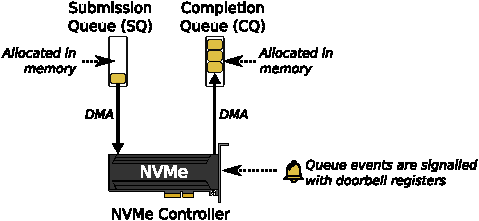
\includegraphics{nvme}
    \caption
    [\Glsfmtshortpl{nvme} support parallel operation by using independent queues. An \glsfmtshort{nvme} uses \glsfmtshort{dma} to fetch commands and post completions]
    {\Glspl{nvme} support asynchronous operation by usingpairs for submitting \gls{io} commands and receiving completions. These queues are hosted in memory, and an \gls{nvme} uses \gls{dma} to fetch commands and post completions.}
    \label{fig:nvme}
\end{figure}



\Cref{fig:nvme} shows how \glspl{nvme} support asynchronous operation by using a system of paired command \glspl{sq} and \glspl{cq}.
%
Both types of queues are data structures that are allocated in memory by discretion of the driver, and may be placed in \emph{any} memory location.
%
The driver submits \gls{io} commands, such as reading or writing $N$ blocks from storage, to an \gls{sq}.
%
The \gls{nvme} will use \gls{dma} to fetch commands from the \gls{sq}, and once a command is carried out, the \gls{nvme} posts the command completion status to the associated \gls{cq} (also using \gls{dma}) containing the status of the command.
%
``\Glspl{db}'' on the \gls{nvme} device are used to signal when new commands should be fetched, and each queue has its own \gls{db}.
%
Furthermore, as \emph{multiple} of these queue pairs can be created, \glspl{nvme} avoid any contention in the command submission and completion paths.
%
An example of this is a multi-core \gls{cpu} that assigns an \gls{sq} and an associated \gls{cq} per \gls{cpu} core, allowing each core to operate the \gls{nvme} independent of others.


\begin{figure}
    \centering
    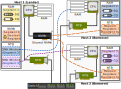
\includegraphics[width=.99\textwidth]{nvme-driver}
    \caption
    [NVMe driver]
    {TODO make caption}
    \label{fig:nvme-driver}
\end{figure}

As shown in \cref{fig:nvme-driver}, our own driver implementation works by taking this one step further, allowing \glspl{cpu} in different machines to operate an \gls{nvme} simultaneously using their own queue pairs.
%
Each machine allocates a \gls{memorysegment} where it sets up the queues' data structures, and uses the \gls{apiext} to map these segments for the device as \glspl{dmawindow}.
%
This allows the \gls{nvme} to read \gls{sq} memory and write to \gls{cq} memory the same way it would access local memory, using native \gls{dma}.
%
Likewise, as \glspl{devicebar} are automatically exported by SmartIO as \glspl{segment}, all machines can memory map \glspl{db} for their respective queues.
%
Since queues are completely parallel, all the machines can submit \gls{io} commands and receive completions entirely independent of each other, once the queues are configured.
%
Note that all machines are able to operate the \gls{nvme} at the same time, including the \gls{lender}.
%
The software is the same regardless of which machine it runs on, as SmartIO keeps track of where the \glspl{segment} and the device reside.



Many \glspl{gpu} support \gls{p2pdma} in order to avoid unnecessary copies via system memory.
%
This makes it possible for \gls{gpu}-accelerated applications that require fast storage to directly load data into \gls{gpu} memory~\cite{Bergman2019,url:Thompson2019}.
%
For Nvidia \glspl{gpu}, it is possible to make on-board \gls{gpu} memory accessible through the \gls{gpu}'s \glspl{bar} using the \gls{gpudirect}~\gls{api}~\cite{url:GPUDirect}.

For Nvidia \glspl{gpu}, \gls{p2pdma} with other devices is supported using their \gls{gpudirect}~\gls{api}~\cite{url:GPUDirect,url:Rosetti2014}.
%



is able to decide where \glspl{segment} should be allocated based on memory access pattern hinting, as explained in \cref{sec:api}.


\begin{figure}
    \centering
    \begin{subfigure}{\linewidth}
        \centering
        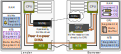
\includegraphics[width=.99\textwidth]{nvme-local-gpu}
        \caption{TODO make caption for local GPU}
        \label{fig:nvme-local-gpu}
    \end{subfigure}
    \par\vspace{5mm}
    \begin{subfigure}{\linewidth}
        \centering
        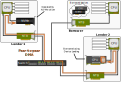
\includegraphics[width=.99\textwidth]{nvme-remote-gpu}
        \caption{TODO make caption for remote GPU}
        \label{fig:nvme-remote-gpu}
    \end{subfigure}
    \caption
    [A caption]
    {TODO make caption for cool GPU stuff}
    \label{fig:nvme-gpu}
\end{figure}


\begin{figure}
    \centering
    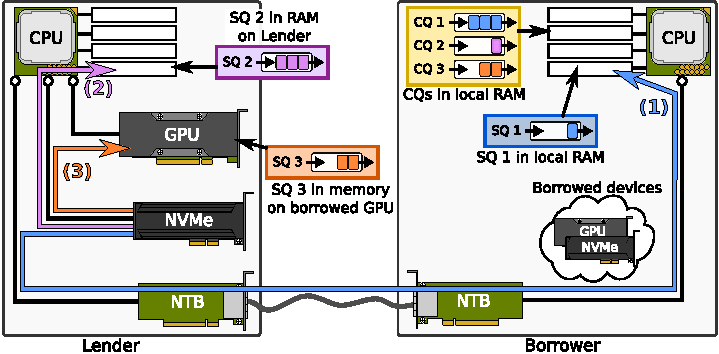
\includegraphics{nvme-queues}
    \caption
    [NVMe queues]
    {TODO make caption for SQ optimization}
    \label{fig:nvme-queues}
\end{figure}





\begin{itemize}
    \item why a prototype driver? demonstrate disaggregation in software
    \item why nvme? easy to parallelize because of queues
    \item driver implementation and queue sharing
    \item gpudirect + co-operation with device lending
\end{itemize}

%We demonstrate this combining with as part of the evaluation of our proof-of-concept \gls{nvme} driver in \paperref{tocs:eval-nvme-sq}.




\section{Performance measurements}\label{sec:eval}
Some selected performance graphs here, demonstrating zero-overhead :)

\section{Related work}\label{sec:rw}
should rw go in discussion and conclusion instead?
\begin{itemize}
    \item rdma stuff
    \item fabric partitioning: mr-iov, broadcom/microsemi chips with partitioning
    \item ladon (and other ntb stuff)
    \item disaggregation
\end{itemize}

